\chapter{Discussion}

\label{ch:discussion}

This chapter interprets the results research question by research question, then turns to the measurement artefacts identified during the study and to the scope of the findings.

\section{Main Findings}

\paragraph{RQ1: What Frozen Frontier Models Can and Cannot
Do}

\label{sec:disc-rq1}

Frozen frontier models write SPARQL that parses and executes but is rarely correct (\cref{sec:res-frozen}, \cref{tab:main}).
On non-empty outputs their scores lie close together.
What separates the systems is mainly how often they return nothing, and the pipeline roughly halves that rate.
Their weakness lies in Wikidata's modelling conventions (statement nodes, subclass closure, normalised value nodes), which they rarely apply where needed.

The failures are shared across models.
Three quarters of the questions are solved by none of the four models, which come from four different organisations.
The questions that all four fail share a clear feature in their reference queries: they contain several times more statement nodes than easier questions, and qualifier access and aggregation, which appear in them, never occur in the questions that all four models solve.
This suggests that the difficulty is a property of the questions themselves.

Fine-tuning brings conformity to a query style, the very capability the frozen models lack: a 7B model trained on in-domain queries scores orders of magnitude higher than a much larger base model.
This does not prove a general difference in capability, since more than half of its outputs are character-identical to the reference, although that alone does not establish leakage.
A fine-tuned system reproduces a distribution of queries, whereas this pipeline derives a query from the question. The two agree only when the reference translates the question correctly, but the audit shows noise in roughly one quarter of the strict fair set.
Whether this contributes materially to the observed gap remains open, since only sixteen adjudicated rows overlap the official split, and it is listed as future work.

The comparison that matters most for this thesis is among systems without in-domain training, and there the pipeline more than doubles the best published frozen result.
The stage-wise analysis also shows where the remaining difference to fine-tuned systems comes from.

\paragraph{RQ2: Why Disambiguation Is Not the
Bottleneck}

\label{sec:disc-rq2}

Given the benchmark's concepts and query structure, the pipeline reaches 97.4 entity-level Jaccard (\cref{sec:res-attribution}, \cref{tab:main}).
When it has to generate the query itself, the score falls to 30.9.
In this pipeline, query generation is the main constraint.
Disambiguation over retrieved candidates stops being the limiting stage once the model writes suitable labels and the correct entity is in the candidate pool, which holds for the frontier model here.
For the small open model, label generation itself becomes the weak point (see RQ3).

Rebuilding the candidate pools with rate-limited retrieval adds further support: the gold-label condition improved roughly ten times more than the end-to-end condition, which is hard to explain if disambiguation were the main constraint.

Structure is the largest single component of the gap and dominates at high complexity, but it is not the only source of error: projection mismatches and residual identifier errors each account for about one fifth of the failures.
Within generation, the factorial arm separates the two decisions: fixing the concepts is worth +19.72 points and naming the required idioms +3.76, and the two effects add up.
Even with both supplied, the model reaches 50.4 against 97.4 for the gold-label condition, so composing the query around the right concepts remains the largest single step.

\paragraph{Performance of the End-to-End Linkers}

The fine-tuned linkers' deficit of about 70 points traces to the mention-detection mismatch discussed in the related work, and the set-based metric closes only a small part of it.
Given the same candidates, the bi-encoder trails the reasoning linker by 24.9 points and the plain search order by about 21, so reasoning over candidates is the strongest of the compared mechanisms, while most of its accuracy comes from labels that Wikidata's search can find.
Research that focuses mainly on entity linking for this task, including the 35.1\,\% failure share reported by \citet{xu2023wikisp}, may therefore be improving a stage that this architecture has largely solved.
\citet{xu2023wikisp} measured a fine-tuned system on simpler questions, where linking makes up a larger share of the errors; the two results describe different architectures and do not contradict each other.
For a pipeline of this kind, better disambiguation offers little headroom, while query generation leaves much more room.

\paragraph{RQ3: What Backbone Scale Buys, and
Where}

\label{sec:disc-rq3}

Backbone dependence differs by stage (\cref{sec:res-linkers,sec:res-backbone}, \cref{tab:linkers}).
At disambiguation, scale has little effect: 97.7 (frontier), 94.9 (14B) and 95.8 (7B) entity F1, with overlapping intervals.
Reasoning over seven retrieved candidates does not need a frontier-scale model.
At generation, however, the choice of backbone matters much more: when the open model handles both stages, pipeline performance drops sharply.

Asked to name Wikidata entities and properties without further help, the open model produces unfindable labels for 16.4\,\% of distinct labels (270 of 1,645), against 3.3\,\% for the frontier model, a 4.9-fold difference.
This points to a hybrid deployment, with a capable model for labels and a cheaper one for disambiguation.
String normalisation, which should fix superficial casing issues such as camelCase or snake\_case, lowers the failure rate only to 13.8\,\%.
The main problem is near-miss wording (``crew member(s)'', for example, names a different property and is not a misspelling), and normalisation hardly touches it.
The replication with Claude Opus 5 repeats generation with a later frontier model and finds the same pattern: subclass closure and property paths improve, statement nodes and qualifiers improve little, and value nodes do not improve.
The generation deficit does not disappear as models get better.
Schema evidence, selective gating, majority voting and string repair fail in the same way: none of them supplies knowledge of how the graph itself names and models information.
The disambiguation results show that the smaller model already reasons well enough for that stage, so the most likely explanation for the generation gap is missing vocabulary knowledge.

\paragraph{RQ4: Guidance versus
Evidence}

\label{sec:disc-rq4}

Generic idiom guidance brings a small benefit (\cref{sec:res-prompts}, \cref{tab:significance}), evidence about graph contents does about four times as much harm, and selective guidance does not beat always-on guidance, even with oracle knowledge of when it is needed.

\paragraph{Overuse of Schema Evidence}

When the model is shown the properties of an entity, it uses them about twice as often as the reference does.
Making the evidence shorter and explicitly conditional does not reduce this overuse but increases it.
The grounded arms share only half as much label vocabulary with the baseline as the idiom arm does.
The intervention failed even though the schema cards were built from reference-linked mentions, with no linking errors at all.

\paragraph{Predicting Construct Need from the Question}

A classifier that predicts from the question text alone whether a reference query uses a given construct reaches only moderate performance (AUC 0.62--0.82).
Its strongest features for subclass closure are topical terms (``libraries'', ``hospitals'', ``scientists''), which describe the subject of a question, not how Wikidata models it.

\paragraph{Cost of Unnecessary Idiom Use}

The idiom prompt helps most when the reference needs the construct it describes, and on average it still raises accuracy when it does not, although individual questions can get worse.
Unnecessary closure over a class without subclasses simply returns the same rows.
Construct predictions are miscalibrated, but the cost in accuracy is small, so selective application addresses a problem that is usually cheap.

\paragraph{Constraining versus Enumerating the Schema}

The contrast with \citet{zhang2026saga} helps explain the schema-evidence result.
SAGA filters candidates by type, domain and range, removing options that would otherwise be chosen wrongly.
The schema-evidence arm does the opposite and adds options, which the model seems to take as encouragement.
The same graph information has opposite effects, depending on whether it filters or merely informs.
This also explains why linking (seven candidates, a forced choice) does better than grounding (everything an entity carries, with no restriction).
The direction of the knowledge mattered more than its amount: narrowing the decision space helped, and widening it hurt.
The same distinction sets this result apart from \citet{yang2026ggc}, whose gate reduces the cost of an expensive and often harmful operation.
The gate tested here would have to improve accuracy for an operation that is cheap and almost never harmful, so there is no comparable gain for gating to find.

\paragraph{Testing the Principle}

The prompt experiment keeps the same reference-linked information and changes only how it is presented.
Offered as available evidence, it lowers performance by 14.65 points.
Imposed as a mandatory closed list, it raises performance by 18.99 points.
The intervals do not overlap, which leaves a difference of about 34 points from framing alone.
The absolute level is partly definitional, because the permitted list is drawn from the reference query's own vocabulary, so the evidence lies in the contrast between the two framings.
The model broke the prompt-level constraint for only 0.7\,\% of label uses.

The mechanical half of the principle was tested separately.
Applying every type constraint declared in Wikidata removes the reference property for 7.5\,\% of the affected mentions, while using only mandatory constraints is safe but has almost no effect.
The principle still holds, since constraining beats enumerating.
A mechanical filter, however, is only as reliable as Wikidata's own assertions, and most declared type constraints are not binding.

\paragraph{What the Interventions Changed}

The constrained arm gains more than the construct-profile arm, because it settles concept selection, the larger of the two generation decisions it can address.
The factorial arm shows that the two contributions add up, and naming a construct is still not the same as providing the composed query.
The profile hint tells the model which idiom a question needs, but it does not show how to build a complete query around it.
General advice brought no further gains in these experiments.
Restricting the identifiers available to the generator was the more effective intervention.

\paragraph{RQ5: Detectable Failure and the Value of
Execution}

\label{sec:disc-rq5}

Some failures can be detected without the gold query (\cref{sec:res-cascade}, \cref{tab:cascade}).
A cascade that accepts the first non-empty, error-free result raises the score by +4.83 points [2.93, 7.08] without any additional training.
Because it only replaces empty or failed results, it cannot worsen a question by design.
Of the 92 fallback rows, 64 are triggered by empty results.
The gain amounts to about two fifths of the 12-point oracle headroom, so execution feedback catches some failures but cannot correct a query that runs successfully and returns the wrong answer.

The cascade also beats result-set majority voting (37.0 vs.\ 33.8 for the centroid, against a 32.2 baseline): agreement between outputs is a weaker signal than execution, because wrong queries can agree with each other.
Unlike agentic self-correction, which generates, executes and revises queries in a loop, the cascade checks existing alternatives in a fixed order.
This makes it cheaper and easier to reproduce.
It recovers a failure whenever one of the alternatives is correct.
Generating the correct structure in the first place remains the main direction for future work.

\section{Methodological
Implications}

\label{sec:disc-artefacts}

Four measurement artefacts arose during the study, each producing a plausible but incorrect intermediate result.
All four were detected and corrected before the final analysis and are documented in the appendix.
Their causes differed, but they had one feature in common: the result was plausible and fitted the emerging interpretation.

\begin{table}[htbp]
\centering
\small
\caption{Four measurement artefacts: the apparent result and the correction.}
\label{tab:artefacts}
\begin{tabular}{@{}p{3.1cm}p{4.6cm}p{5.6cm}@{}}
\toprule
Artefact & Apparent result & Correction \\
\midrule
Jaccard(\(\emptyset\),\(\emptyset\)) = 1 & Inflated the score of systems that returned nothing & Strict fair set requires a non-empty reference \\
Silent API throttling & An 80.4\,\% candidate ceiling read as a retrieval bottleneck & Rate-limited, repaired pools raised the ceiling to 99.4\,\% \\
Exceptions caught as empty strings & A reported 66.8\,\% generation-success rate on complex questions & Every affected row succeeded on regeneration \\
A stale error sample & Complex failures judged to contain no linking errors & The correct run contained three linking errors among fifteen \\
\bottomrule
\end{tabular}
\end{table}

The lesson is that a plausible result needs more than a check of the final score: these artefacts were caught through regeneration, auditing and comparison with intermediate outputs.
In practice, empty or unusually short responses from the Wikidata search API should be treated as suspicious and re-checked with repeated requests, and KGQA experiments should be regenerated end to end from stored inputs after any change to the pipeline.

\begin{figure}[htbp]
  \centering
  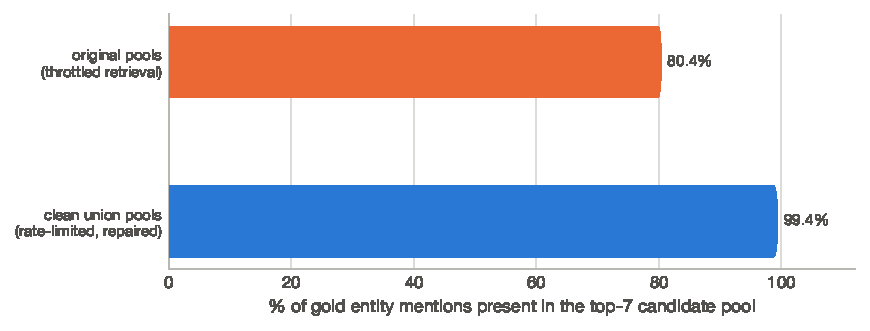
\includegraphics[width=0.88\textwidth]{figures/fig_candidate_ceiling.pdf}
  \caption{A measurement artefact: the candidate ceiling before and after pool repair.}
  \label{fig:ceiling}

\end{figure}

\emph{Figure note}.
The initial 80.4\,\% ceiling was caused by silent API throttling.
The issue came to light through rank analysis and through the implausibly large improvement after the pools were repaired.

\section{Limitations and Scope}

\label{sec:limitations}

\begin{enumerate}
\def\labelenumi{\arabic{enumi}.}
\item
\textbf{Evaluation asymmetry.}
The reasoning linkers and GLiNKER receive mention strings and curated candidate lists, whereas ELQ and ReFinED have to detect mentions themselves.
The set-based metric closes part of this gap (+5.4 and +6.8 points), and GLiNKER is evaluated on the reasoning linker's candidate lists rather than with its own retrieval.
\item
\textbf{Benchmark validity.}
Reference noise affects an estimated 24.6\,\% of the strict fair set (interval [12.9, 42.0]).
Scores are not corrected for it, so that they remain comparable with the existing literature.
\item
\textbf{Scope.}
The study evaluates four models from four organisations and two frontier generations in an English setting, on one Wikidata dump served by QLever, which excludes around 15\,\% of gold queries that depend on Blazegraph-specific behaviour.
The linking results are replicated on LC-QuAD 2.0, while the structural gap is measured on Instruct-to-SPARQL.
The design principle of constraining rather than enumerating the schema is established on one benchmark, one generation backbone and one schema-card design.
\item
\textbf{Oracle interventions.}
The constrained-vocabulary and construct-profile arms draw their information from the reference query, and the permitted list can also hint at structure, for example when it contains a qualifier property.
\item
\textbf{Cascade assumptions.}
The cascade never lowers accuracy on the strict fair set because every reference returns a result.
Where an empty answer can be correct, an empty result is not always a failure.
Its prompt order was chosen from the relative quality of the runs, and the split-half evaluation shows that the gain holds when the order is chosen on other questions.
\item
\textbf{Sample size of the error analysis.}
The error taxonomy covers 30 failures and identifies recurring types rather than population frequencies.
The corpus-wide construct analysis across all 567 rows supports the same conclusion.
\end{enumerate}
